\chapter{Komprese dat}
Komprese nebo také komprimace dat je taková transformace dat, která má za cíl úsporu zdrojů při ukládání nebo archivaci a nebo snížení datového toku při přenosu, to vše při současném zachování informace obsažené v datech. Jinými slovy jde o redukci velikosti datových souborů, jehož následkem je úspora paměťových či přenosových kapacit. Postup, při kterém z komprimovaných dat rekonstruujeme data originální, se nazývá dekomprese.

\section{Princip komprese dat}
\label{sekcePrincipKompreseDat}
Data velmi často obsahují tzv. redundantní\footnote{Redundance znamená informační nadbytek, např. vícenásobný výskyt slov v textu.} informaci, toho právě využívá komprese -- data jsou zpracována tak, aby byla redundance minimalizována. Jak lze vidět na obrázku \ref{kompreseDekomprese}, je na vstupní data použita operace komprese. Operací dekomprese dostaneme poté data rekonstruovaná -- v závislosti na použité kompresní metodě, respektive na požadavcích získáme buď data přesně odpovídající původním a nebo pouze částečná. Z tohoto hlediska rozlišujeme dva typy kompresních metod: ztrátové a bezeztrátové.

\begin{figure}[!htb]
\centering
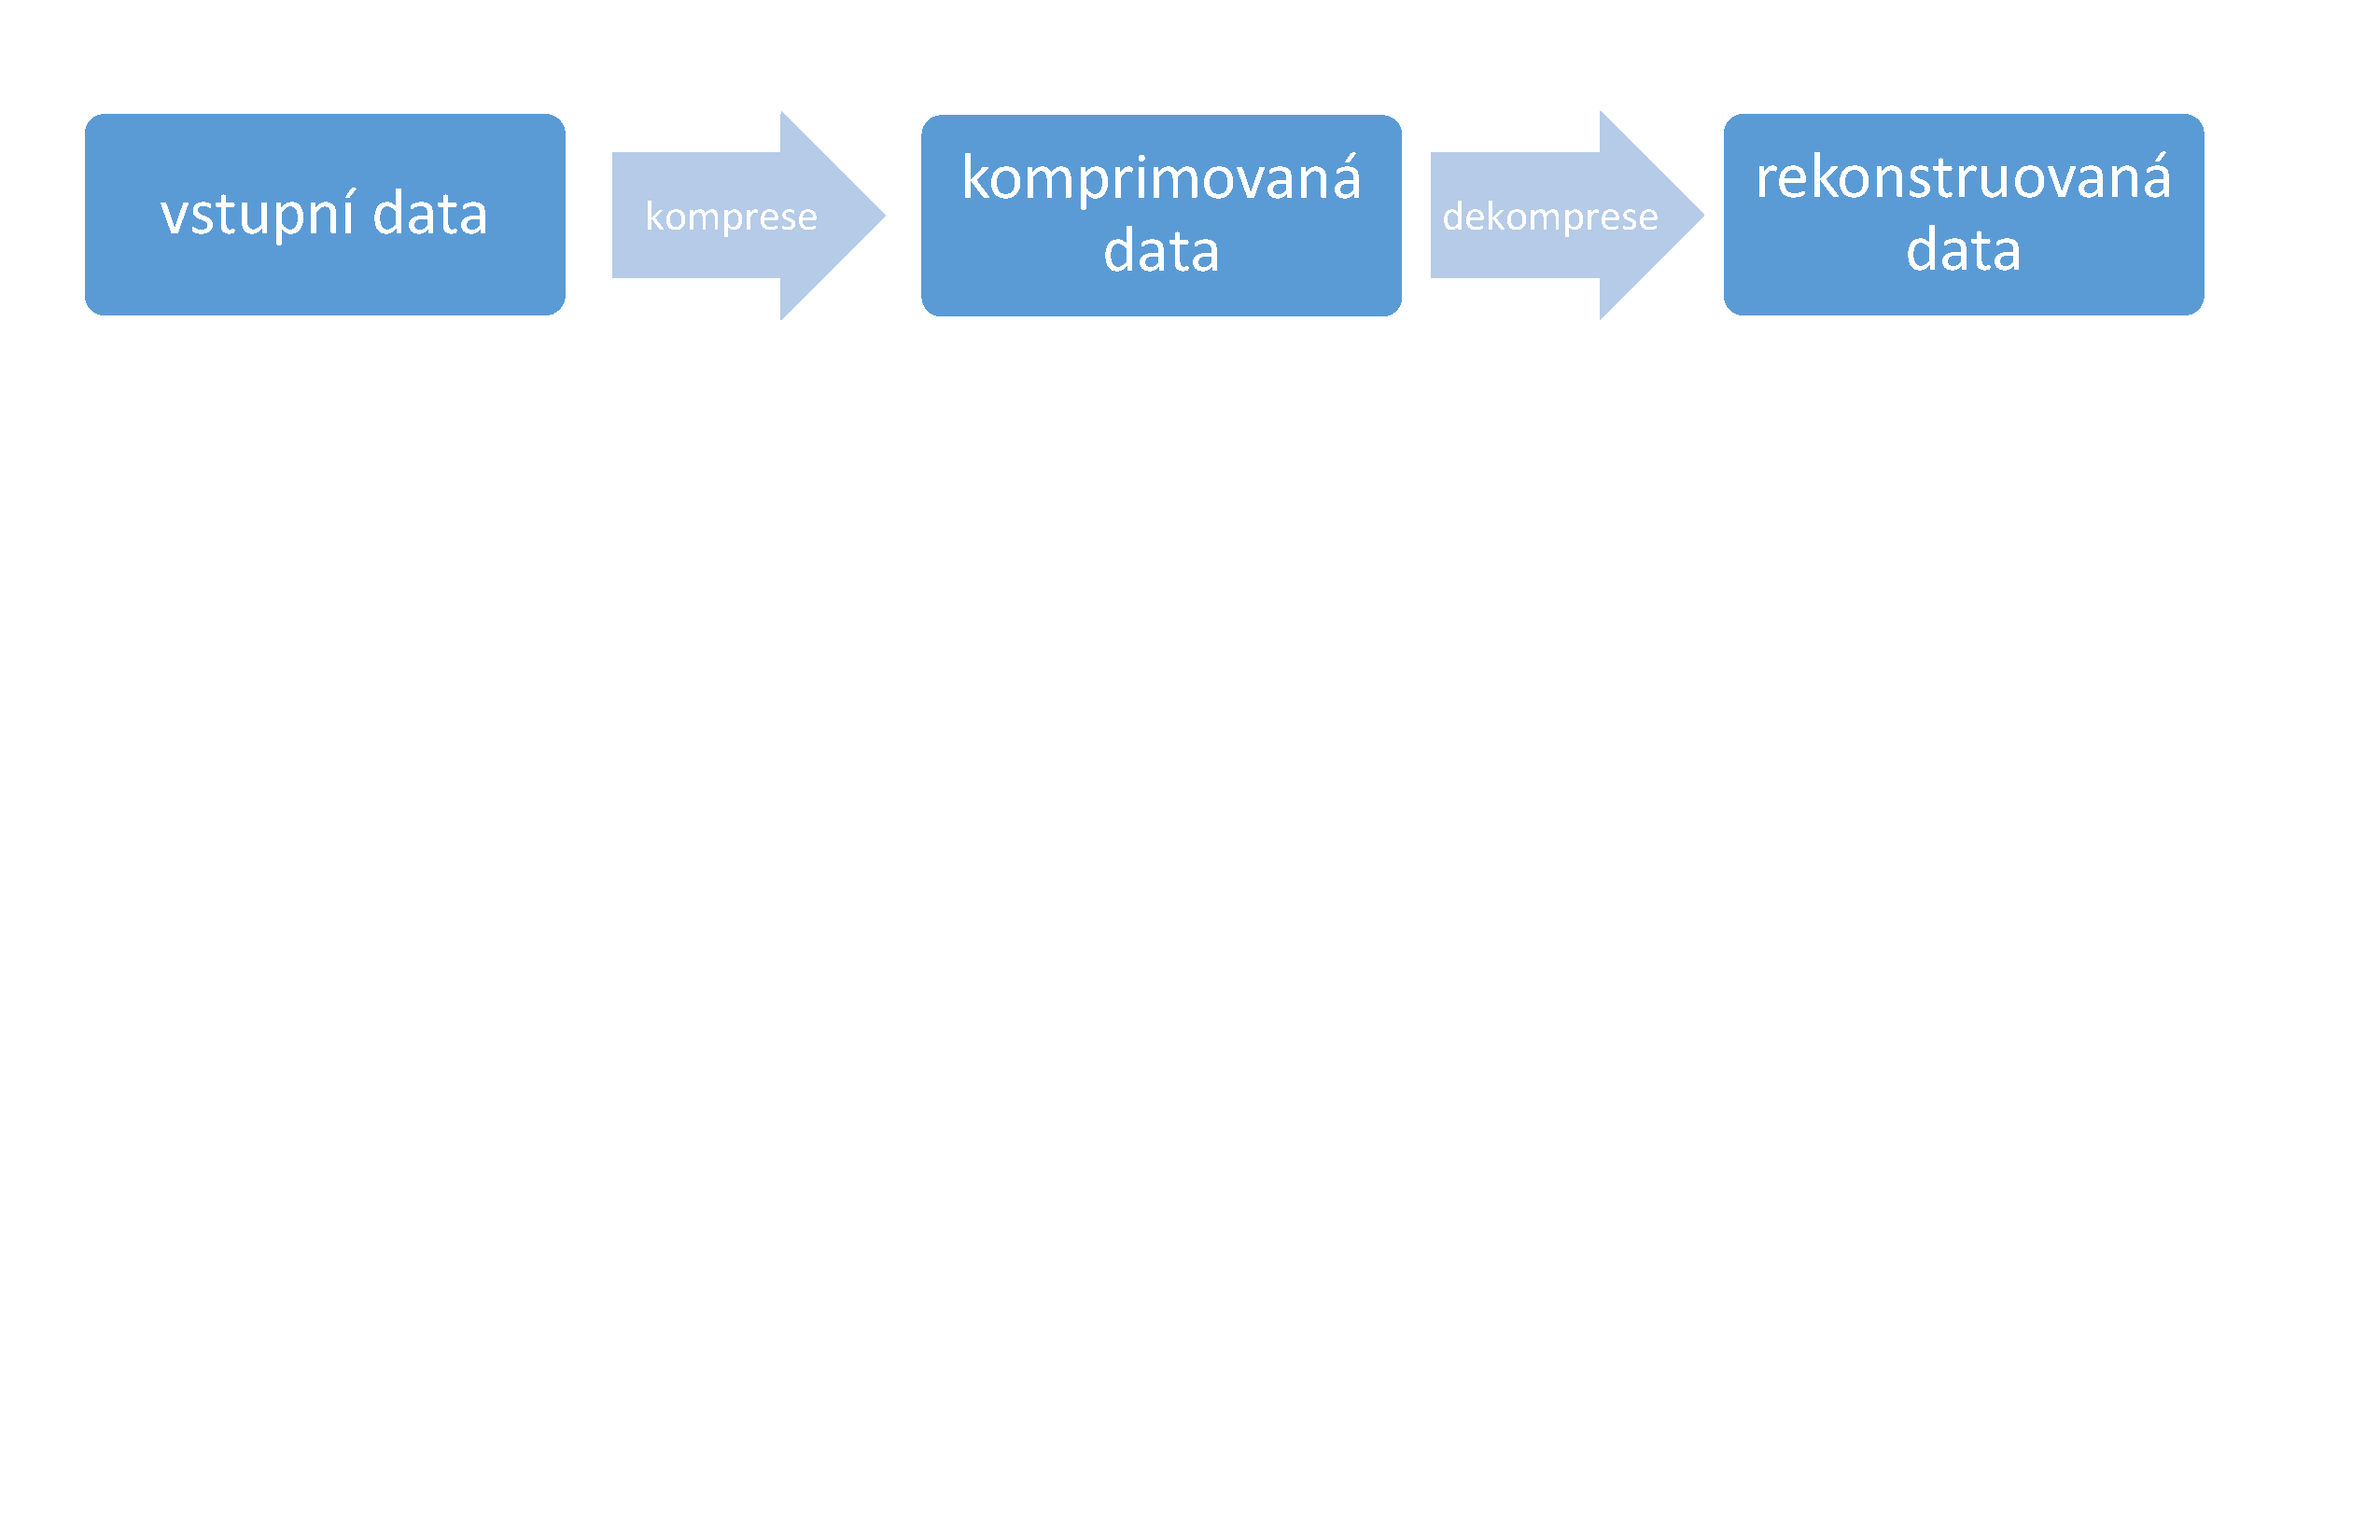
\includegraphics[trim=0 610 60 55, clip, angle=0, width=150mm]{kompreseDekomprese}
\caption{Princip komprese}
\label{kompreseDekomprese}
\end{figure}

\section{Typy kompresních metod}
Jak název napovídá, při ztrátové kompresi ztratíme část informace obsaženou v původních datech, respektive jsou původní data pouze aproximována.  Toto nám nemusí vadit například u obrázků, zvuku a videí, kde je využito nedokonalosti lidských smyslů. Lidské ucho nedokáže například slyšet velmi vysoké frekvence. Má smysl v datech určených k poslechu zachovávat informaci, kterou nemůže člověk slyšet? Častá odpověď je \uv{ne}. Tohoto principu využívá mnoho kompresních metod, například známý zvukový formát MP3. Odstraněním \uv{nepotřebné} informace z dat je dosaženo ještě větší redukce objemu. 

Naopak v případě bezeztrátových metod je při kompresi zachována veškerá informace a při dekompresi
jsou rekonstruována původní data. Těchto metod se využívá převážně tam, kde není možné původní data jakkoliv pozměnit. Například data ve formátech XML a JSON, kterým se věnuji v této práci, si nemůžeme dovolit pozměnit (přestanou mít původní význam), nebo dokonce ztratit.

\section{Charakteristika komprese}
Kompresní algoritmy lze hodnotit z mnoha různých úhlů pohledu. Můžeme měřit složitost algoritmu, rychlost, jakou jsou data komprimována a dekomprimována (to může být ovlivněno výkonem stroje, na kterém algoritmus běží), jak moc odpovídají rekonstruovaná data původním atd.
Jednou z nejčastějších charakteristik je, logicky ze smyslu komprese vy\-plý\-va\-jí\-cí, tzv. kompresní poměr, který vyjadřuje velikost komprimovaných dat vůči původním, lze ho zapsat následujícím  vztahem:
\begin{equation}
\texttt{kompresní poměr} = \frac{\texttt{délka původních dat}}{\texttt{délka komprimovaných dat}}.
\end{equation}

Další sledovanou charakteristikou je tzv. úspora místa, která je vyjádřena jako:
\begin{equation}
\texttt{úspora místa} = \texttt{1 - kompresní poměr$^{-1}$}.
\end{equation}

Mějme například 2D obrázek o velikosti $256\times256$ pixelů, který zabírá 65536 bytů. Obrázek zkomprimujeme a zabírá-li komprimovaná verze 16384 bytů, můžeme říct, že kompresní poměr je $4:1$ a úspora místa 75 \%. 

\section{Míra informace v datech}
Než se budeme moci věnovat jednotlivým kompresním metodám, připomeňme stručně myšlenky z teorie informace, které poskytly základ pro rozvoj metod bezeztrátové komprese. V této části předpokládám čtenářovu znalost základů teorie pravděpodobnosti a statistiky.

Informační entropie\footnote{Nazývaná též jako Shannonova po Claudu E. Shannonovi, který zformuloval klíčové poznatky.}, jakožto míra neurčitosti v datech, nám pomůže lépe porozumět principům komprese. Představme si dva zdroje (označím je $\mathbf{Z}_1$ a $\mathbf{Z}_2$), které produkují zprávy složené ze symbolů (znaků) zdrojové abecedy $\mathbb{A} = \{\alpha, \beta, \gamma, \delta\}$. Oba zdroje generují znaky zprávy náhodně, pro zdroj $\mathbf{Z}_1$ však platí, že mají všechny znaky stejnou pravděpodobnost výskytu a to 25 \%. Pro zdroj $\mathbf{Z}_2$ jsou pravděpodobnosti výskytu popsány v tabulce \ref{pstVyskytu}. Který ze zdrojů produkuje více informace?

\begin{table}[!htb]
\centering
\begin{tabular}{|c|c|}
\hline
Znak & Pravděpodobnost výskytu\\
\hline
$\alpha$ & $p_\alpha = 50\ \%$\\
$\beta$ & $p_\beta = 30\ \%$\\
$\gamma$ & $p_\gamma = 10\ \%$\\
$\delta$ & $p_\delta = 10\ \%$\\
\hline
\end{tabular}
\caption{Pravděpodobnost výskytu znaků abecedy $\mathbb{A}$ ve zdroji $\mathbf{Z}_2$}
\label{pstVyskytu}
\end{table}

Claude E. Shannon si tuto otázku položil následujícím způsobem. Jaký je nejmenší počet otázek s odpověďmi ano nebo ne, které musíme zodpovědět, abychom byli schopni rozhodnout, jaký je následující znak každého zdroje? Odpovědí na tuto zdánlivě složitou otázku je vyhledávací algoritmus binární vyhledávání. Nejefektivnějším způsobem je v každém kroku položit takovou otázku, která rozdělí prohledávaný interval na dvě poloviny z hlediska pravděpodobnosti. Pro zobrazení, jaké otázky pokládat a v jakém pořadí, můžeme využít binární rozhodovací stromy (viz obrázky \ref{rozhodovaciStromZ1} pro zdroj $\mathbf{Z}_1$ a \ref{rozhodovaciStromZ2} pro zdroj $\mathbf{Z}_2$). Čteme je zleva doprava, v uzlech jsou otázky, hrany odpovídají odpovědím a v listech jsou příslušné znaky.

\begin{figure}[!htb]
\centering
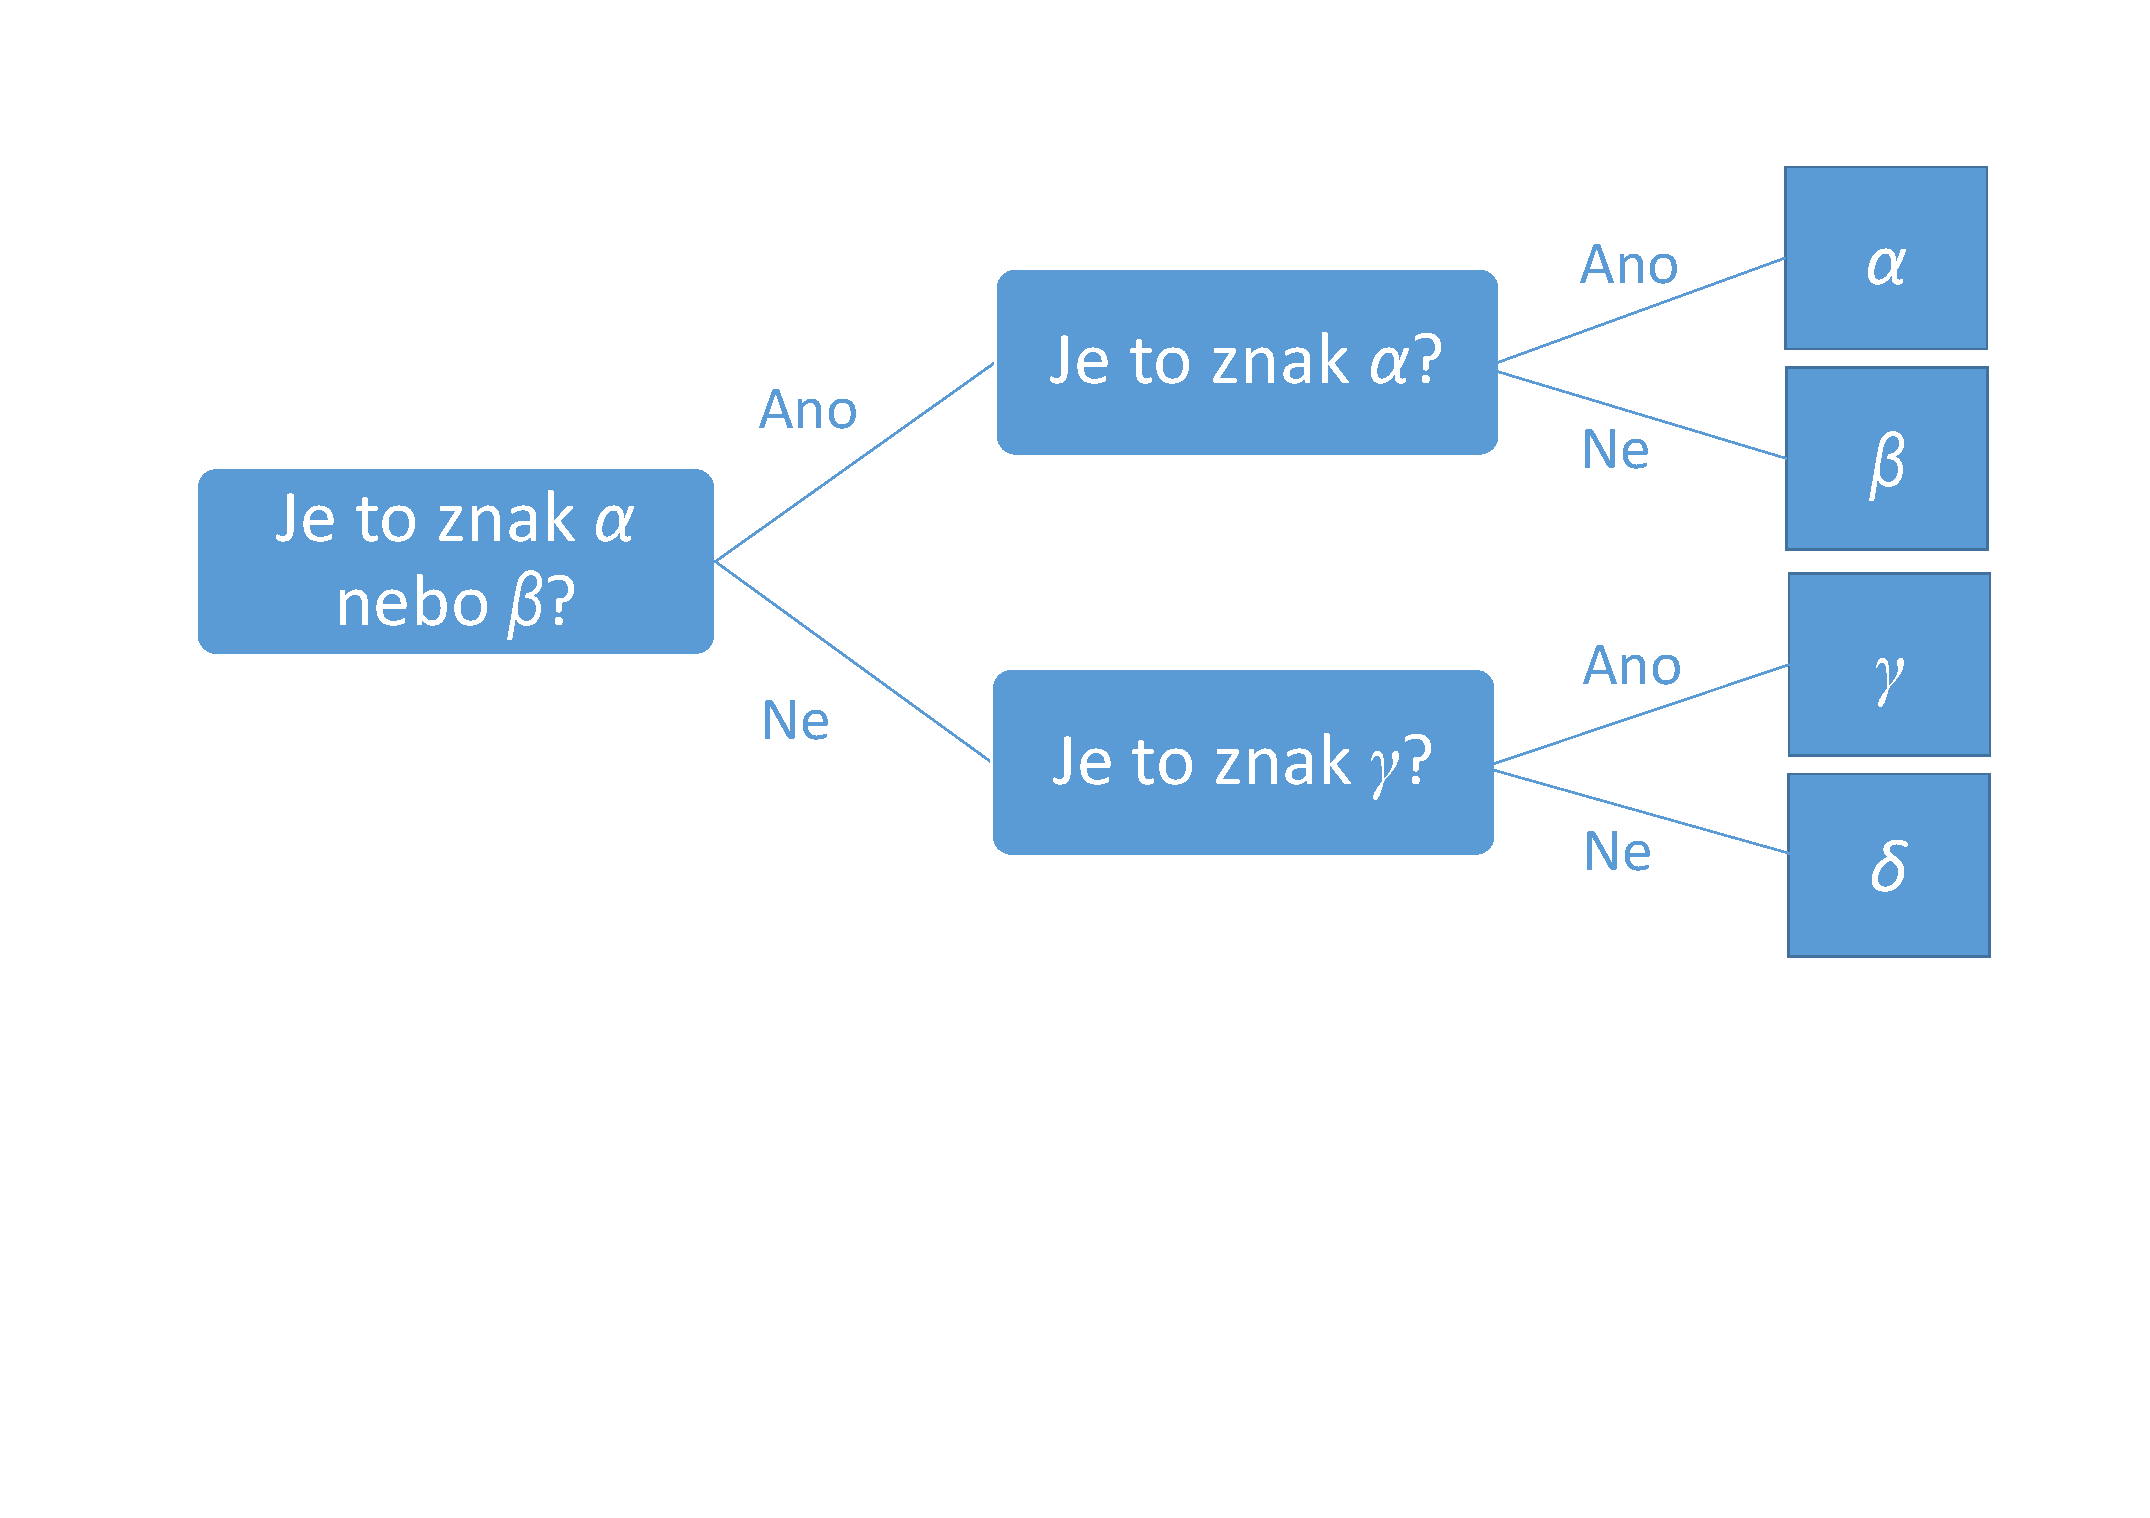
\includegraphics[trim=50 270 50 70, clip, angle=0, width=150mm]{rozhodovaciStromZ1}
\caption{Binární rozhodovací strom pro zdroj $\mathbf{Z}_1$}
\label{rozhodovaciStromZ1}
\end{figure}

\begin{figure}[!htb]
\centering
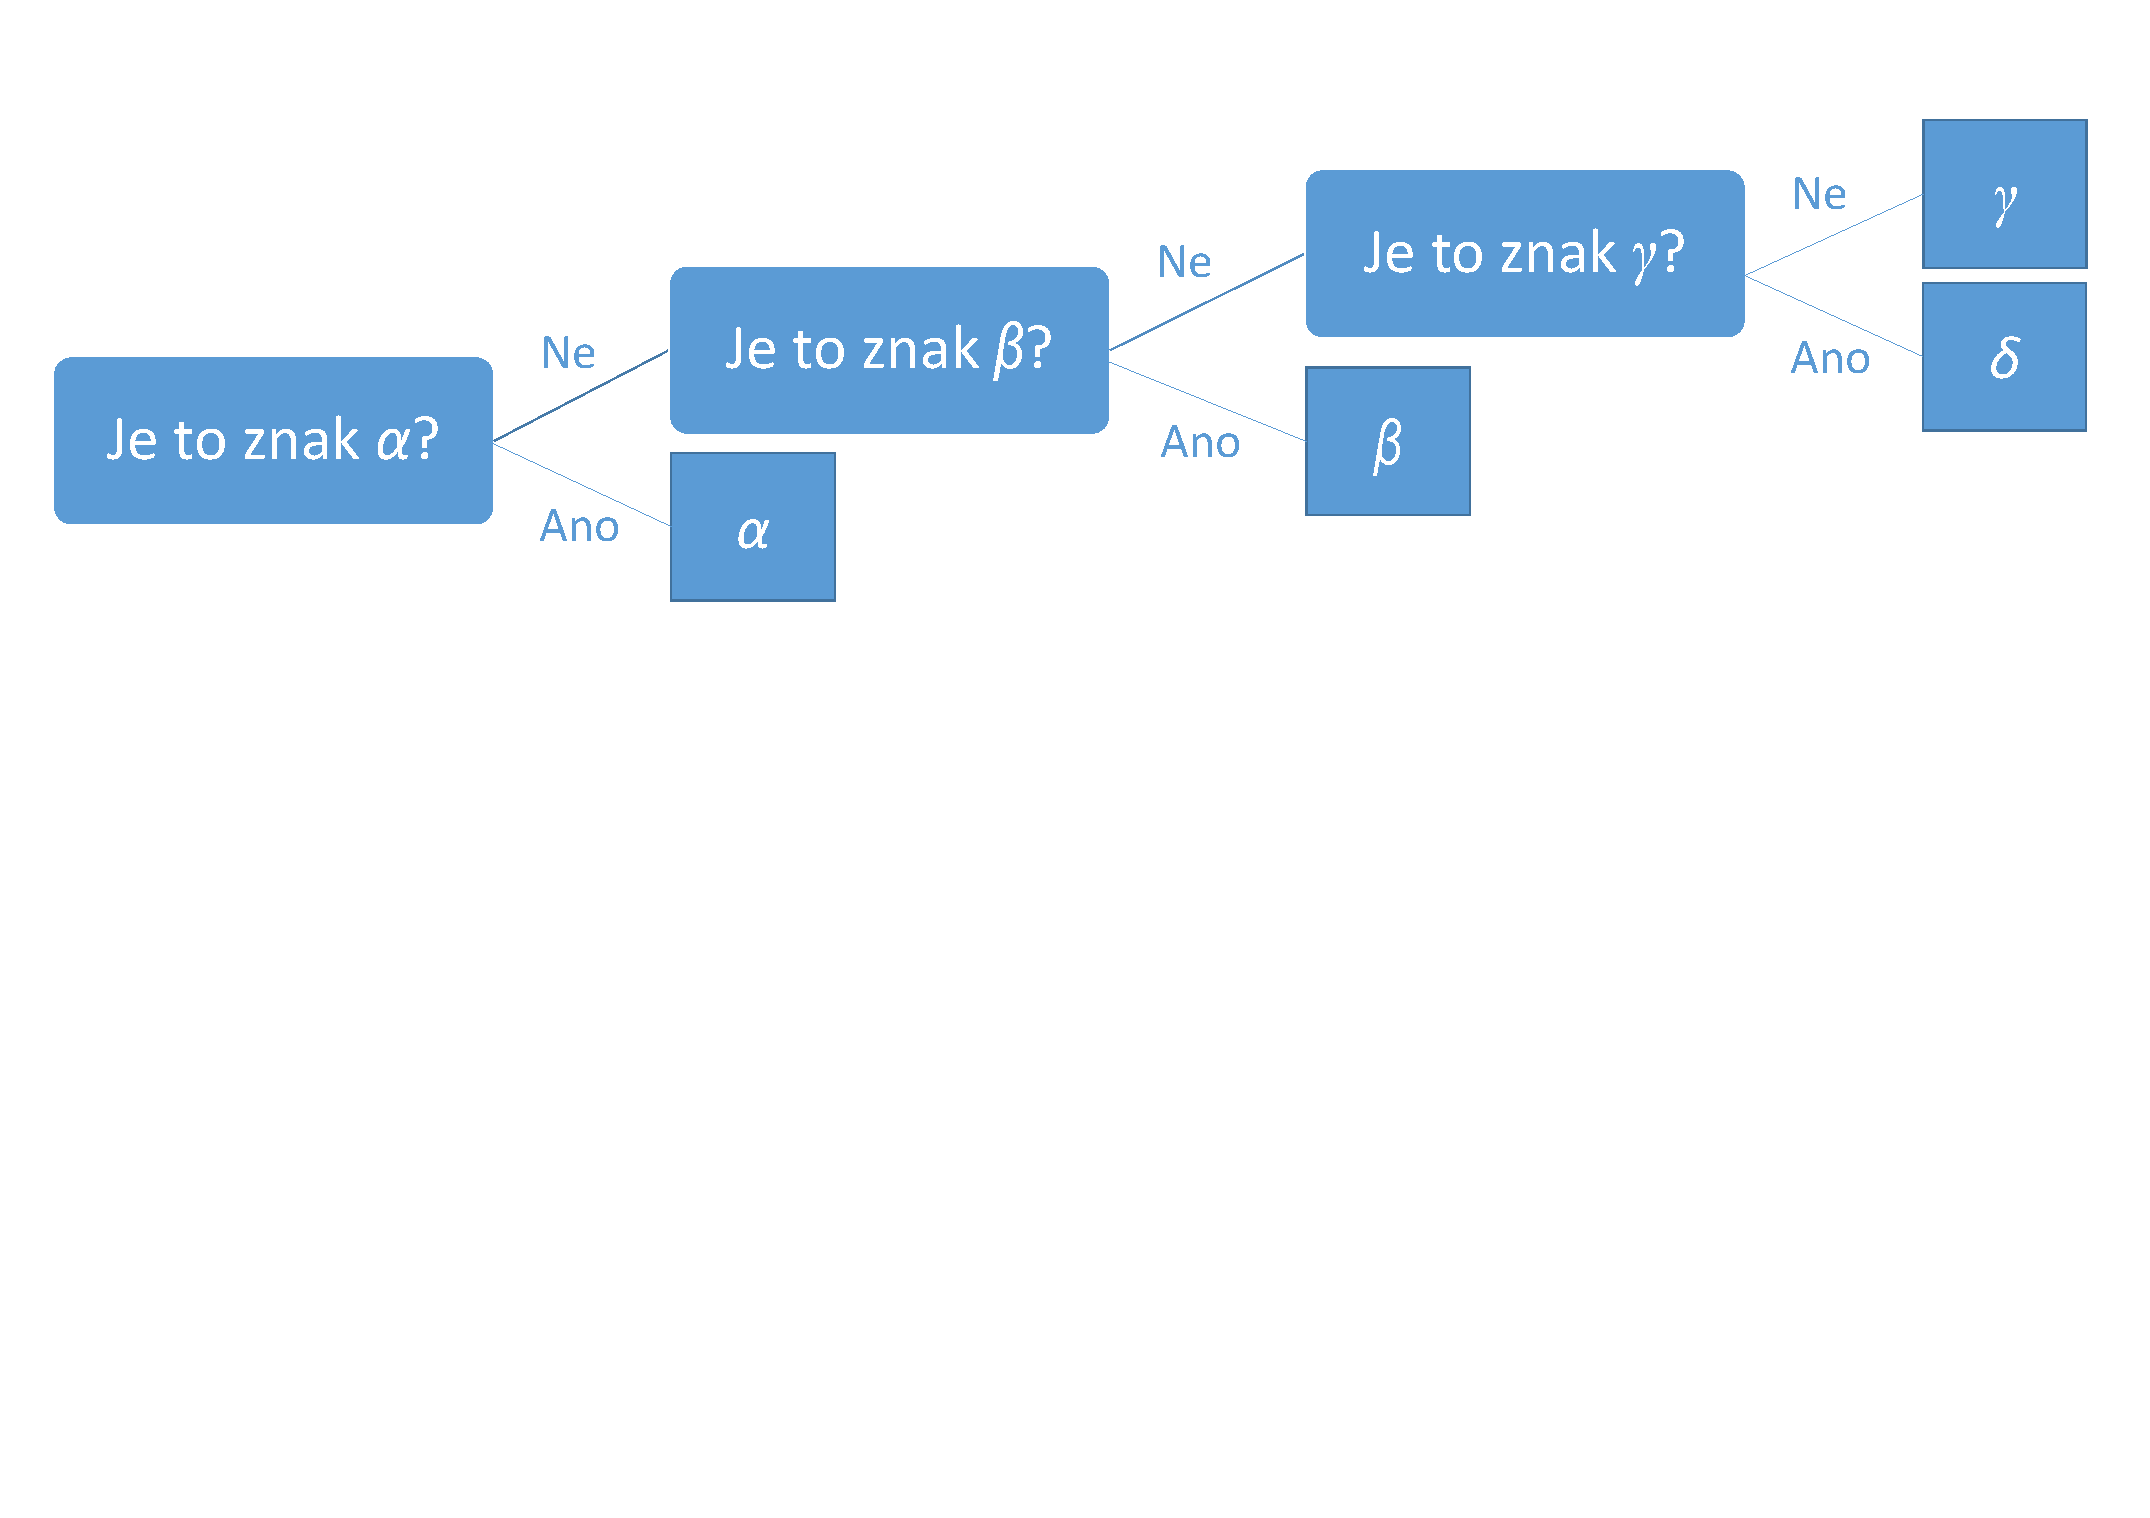
\includegraphics[trim=20 420 20 40, clip, angle=0, width=150mm]{rozhodovaciStromZ2}
\caption{Binární rozhodovací strom pro zdroj $\mathbf{Z}_2$}
\label{rozhodovaciStromZ2}
\end{figure}

Průměrný počet otázek na zjištění jednoho znaku (tento počet označím $\bar{q}$) pokládaných tímto způsobem odpovídá pravděpodobnostem výskytu jednotlivých znaků a lze jej vypočítat jako $\bar{q} = \sum_{a \in \mathbb{A}} \#a \cdot p_a$, kde $\#a$ je počet otázek pro zjištění, že jde o znak $a$, a $p_a$ je pravděpodobnost výskytu znaku $a$. Tedy pro zdroj $\mathbf{Z}_1$ dostaneme $\bar{q}_1 = 2p_\alpha + 2p_\beta + 2p_\gamma + 2p_\delta =2\cdot0,25 + 2\cdot0,25 + 2\cdot0,25 + 2\cdot0,25 = 2$, tedy 2 otázky na znak, a pro zdroj $\mathbf{Z}_2$ dostaneme podobně $\bar{q}_2 = 1p_\alpha + 2p_\beta + 3p_\gamma + 3p_\delta =1\cdot0,5 + 2\cdot0,3 + 3\cdot0,1 + 3\cdot0,1 = 1,7$, tedy 1,7 otázky na znak.

To znamená, že budeme-li se ptát na 1000 znaků u obou zdrojů, budeme muset položit 2000 otázek ke zjištění znaků ze zdroje $\mathbf{Z}_1$ a 1700 otázek ke zjištění znaků ze zdroje $\mathbf{Z}_2$. Výstup zdroje $\mathbf{Z}_2$ obsahuje méně překvapení, nebo lépe neurčitosti, než výstup zdroje $\mathbf{Z}_1$. Hovoříme o tom, že výstup zdroje $\mathbf{Z}_2$ poskytuje méně informace než výstup zdroje $\mathbf{Z}_1$.

\subsection{Entropie informačního zdroje}
V Shannonově teorii je definice zdroje informace prakticky totožná s definicí pravděpodobnostního prostoru, tj. trojice $(\mathcal{X},\mathcal{S},p)$, kde $\mathcal{X}$ je množina elementárních jevů (zpráv), $\mathcal{S}$ je třída náhodných jevů ($\sigma$-algebra podmnožin $\mathcal{X}$) a $p$ je pravděpodobnostní míra na $\mathcal{S}$. \cite{teorieInformace}

Pro nás bude modelem zdroje informace diskrétní pravděpodobnostní prostor $(\mathcal{X},p(x))$, který generuje zprávu $X$, jež je náhodnou veličinou s výběrovým prostorem $(\mathcal{X}, px(x))$. Mezi zprávou $X$ a zdrojem $(\mathcal{X}, p(x))$ panuje ekvivalence, značíme $X \thicksim (\mathcal{X}, p(x))$. Základním pojmem teorie informace je entropie $H(X)$ zdroje $X$, jde o číslo, kterým charakterizujeme, jak obtížné je předpovědět hodnotu dané náhodné veličiny $X$, tj. zprávu, kterou vyprodukuje daný zdroj informace $X \thicksim (\mathcal{X}, p(x))$. Následuje formální definice entropie. \cite{teorieInformace}

\begin{defi}
Entriopie zdroje informace $X \thicksim (\mathcal{X}, p(x))$ je veličina $$H(X) = -\sum_{x \in \mathcal{X}} p(x)\log p(x),$$ kde $0 \log 0 = \lim_{t \to 0_+} t \log t = 0$.
\end{defi}

\subsection{Entropie a komprese}
Když chceme (nejen) komprimovat digitální data, musíme je rozdělit na malé kousky, např. obrázek na pixely, textová data na znaky. To nám umožní zpracovat tato data jako posloupnost symbolů. Jednotlivé symboly pak můžeme reprezentovat s použitím nějakého kódu. Umíme-li zprávy vysílat a přijímat pouze v binární soustavě, vytvoříme kód\footnote{Takové kódy provází lidstvo od nepaměti, např. kouřové signály, Morseova abeceda, reprezentace dat v počítačích atd.} složený ze znaků kódové abecedy $\mathbb{B} = \{0,1\}$.

Vraťme se nyní zpět k abecedě $\mathbb{A}$ a představme si zdroj $\mathbf{Z}$, který generuje zprávy složené ze znaků abecedy $\mathbb{A}$. Tento zdroj má pravděpodobnosti výskytu jednotlivých znaků odpovídající zdroji $\mathbf{Z}_2$, což my zatím ale nevíme. Jako příklad můžeme mít za úkol komprimovat text obsahující 1000 znaků vygenerovaných zdrojem $\mathbf{Z}$. V takovém případě intuitivně přiřadíme jednotlivým zdrojovým znakům nejkratší možná kódová slova viz kód $\kappa_1$ v tabulce \ref{kodovaSlovaZ1}. Tato slova mají délku 2, což znamená, že potřebujeme průměrně 2 bity na znak. 

\begin{table}[!htb]
\centering
\begin{tabular}{|c|l|}
\hline
Zdrojový znak & Kódové slovo\\
\hline
$\alpha$ & 11\\
$\beta$ & 10\\
$\gamma$ & 01\\
$\delta$ & 00\\
\hline
\end{tabular}
\caption{Kód $\kappa_1$ pro zdroj $\mathbf{Z}_1$}
\label{kodovaSlovaZ1}
\end{table}

Pokud analýzou zdroje $\mathbf{Z}$ ale zjistíme, že pravděpodobnosti výskytu odpovídají zdroji $\mathbf{Z}_2$ (viz tabulka \ref{pstVyskytu}), můžeme znakům přiřadit jiná kódová slova (viz tabulka \ref{kodovaSlovaZ2}, která budou brát ohled na nové pravděpodobnosti výskytu. Tento kód $\kappa_2$ je tzv. Huffmanův kód (viz kapitola 3 v \cite{teorieKodovani}) a potřebuje průměrně 1,7 bitu na znak, způsob jeho vytvoření je popsán v části \textcolor{red}{reference na Huffmanovo kódování} nebo v \cite{teorieKodovani}.

\begin{table}[!htb]
\centering
\begin{tabular}{|c|l|}
\hline
Zdrojový znak & Kódové slovo\\
\hline
$\alpha$ & 1\\
$\beta$ & 01\\
$\gamma$ & 000\\
$\delta$ & 001\\
\hline
\end{tabular}
\caption{Kód $\kappa_2$ pro zdroj $\mathbf{Z}_2$}
\label{kodovaSlovaZ2}
\end{table}

Podíváme-li se na obrázky \ref{rozhodovaciStromZ1} a \ref{rozhodovaciStromZ2} a příslušný výpočet průměrného počtu otázek na zjištění znaku, můžeme vidět jisté souvislosti. Například když slova Ano, resp. Ne na hranách rozhodovacího stromu nahradíme čísly 1, resp. 0, dostaneme čtením od kořene k listům odpovídající kódová slova. Stejně tak průměrný počet otázek na zjištění znaku odpovídá střední délce zvoleného kódování (viz definice 7 v \cite{teorieKodovani}).

K jaké úspoře dojde? K zakódování 1000 znaků výše zmíněného textu pomocí kódu $\kappa_1$ potřebujeme 2000 bitů, ale při použití kódu $\kappa_2$ nám bude stačit pouze 1700 bitů. Úspora je tedy 300 bitů. Na otázku, zda je možné tuto úsporu ještě zvýšit, nelze odpovědět jenom ani nebo ne. Pokud zkrátíme délku některých kódových slov v kódu $\kappa_2$, stane se zakódovaná zpráva dvojznačnou a zpětně nedekódovatelnou. Kódujme například znak $\delta$ kódovým slovem 0, potom sekvence 01 může znamenat jak $\delta\alpha$, tak i $\beta$. Abychom odstranili tento problém, museli bychom mezi kódová slova vložit oddělovač, čímž ale zakódovanou zprávu prodloužíme a k požadované úspoře nedojde.

Již Claude E. Shannon tvrdil, že komprese má limit a tím je vždy entropie zdrojové zprávy. Čím je entropie nižší, tím vyšší je možnost komprese. Naopak čím je entropie vyšší, kvůli nepředvídatelnosti, schopnost komprese se snižuje. Pokud bychom chtěli komprimovat až za tento limit, museli bychom nutně část informace vypustit, což je ale přesně princip ztrátové komprese, kterou si nemůžeme vždy dovolit.